The Grover Algorithm was implemented by using multiple classes to represent elements within the algorithm. One such class is the \emph{GroverOracle} this is the equivalent to the Oracle in the Grover Iteration stage. The \emph{GroverOracle} contains the answer that the QRegister will be converged to and also supplies information about the answer, i.e. the number of qubits required to represent it in binary and the base count(\(2^n\)). We chose this design of the Oracle to semantically seperate it from Grover's Algorithm implementation.

Grover's Algorithm is implemented using two different approaches, \emph{GroverDiffusionAlgorithm} with an analytic approach using a matrix as a diffusion operator\cite{solca2008} and \emph{GroverOptAlgorithm} with a combintation of basewise operators to act on the \emph{QRegister}. Both of these implementation only differentiate in the second stage of the algorithm. \emph{GroverOptAlgorithm} is a more efficent implementation due to less memory usage of the operators and is more sequential and therefore less complex to understand.

As a final addition to the Grover's algorithm implementation we added \emph{GroverDisplay} to show the convergence towards the given answer from the \emph{GroverOracle}. The two dimensional basis that is shown is generated by a Gram-Schmidt orthogonalisation of the answer base and initial zero base. The varying colours in the graph represents different steps in the algorithm with the most recent step colored red. As shown the algorithm begins at the superposition base and rotates towards the final answer base.

\begin{figure}[H]
	\centering
	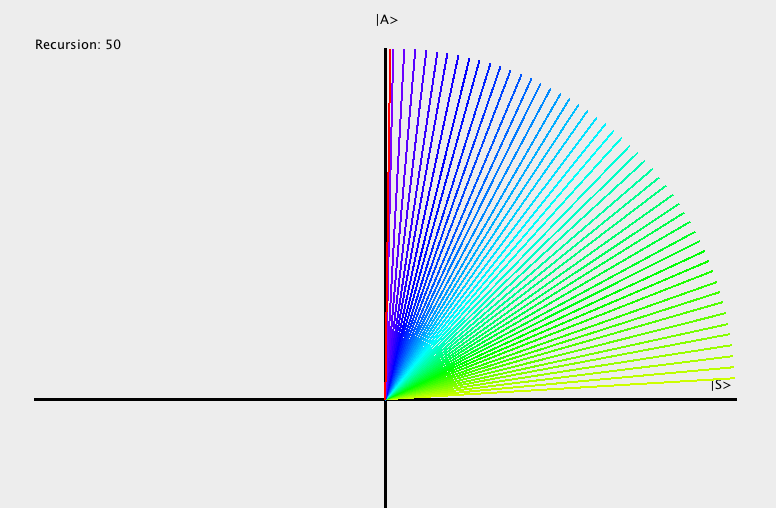
\includegraphics[width=80mm]{./images/GUI}
	\caption{GUI produced from \emph{GroverDisplay}. }
\end{figure}
